\documentclass{article}


\usepackage[final, nonatbib]{neurips_2023}

\usepackage[utf8]{inputenc} % allow utf-8 input
\usepackage[T1]{fontenc}    % use 8-bit T1 fonts
\usepackage{hyperref}       % hyperlinks
\usepackage{url}            % simple URL typesetting
\usepackage{booktabs}       % professional-quality tables
\usepackage{amsfonts}       % blackboard math symbols
\usepackage{nicefrac}       % compact symbols for 1/2, etc.
\usepackage{microtype}      % microtypography

\usepackage{graphicx}
\usepackage{caption}
\usepackage{subcaption}
\graphicspath{{images/}}
\usepackage{multirow}
\usepackage[table,xcdraw]{xcolor}
\usepackage{subfiles} % Best loaded last in the preamble


\title{Feature Manipulating for DDPM based Change Detection}


\author{%
  Daehyeon Choi\\
  20210716\\
  \And
  Jeongho Son\\
  20210979\\
  \And
  Seunghun Oh\\
  20190439\\
}


\begin{document}


\maketitle

\begin{abstract}
  Change Detection is a classic task of computer vision that receives a bi-temporal image pair as an input and separates the semantically changed and unchanged regions of it. Diffusion Model is not only used in Image Synthesis, but also used as a feature extractor and has been applied to various downstream tasks. Using this, a feature map is extracted from the pre-trained diffusion model from the large-scale data set and changes are detected through the additional network in previous. 
  On the one hand, the current Diffusion-based Change Detection approach focuses only on how to extract a good feature map with the Diffusion Model, and obtains and uses difference without further adjustment to the created feature map. Our method focuses on manipulating the feature map extracted from the Diffusion Model to be more semantically useful, and for this, we propose two methods: Feature Attention and FDAF. Our model with Feature Attention achieved state-of-the-art F1 score(91.52) and IoU(84.36) on LEVIR-CD dataset. All our codes are available at \href{https://github.com/choidaedae/POSTECH-CSED538/}{https://github.com/choidaedae/POSTECH-CSED538/}.
\end{abstract}


\section{Introduction}

\subfile{subfiles/introduction.tex}


\section{Method}

\begin{figure}[h]
  \centering
  \begin{subfigure}[b]{0.4\linewidth}
      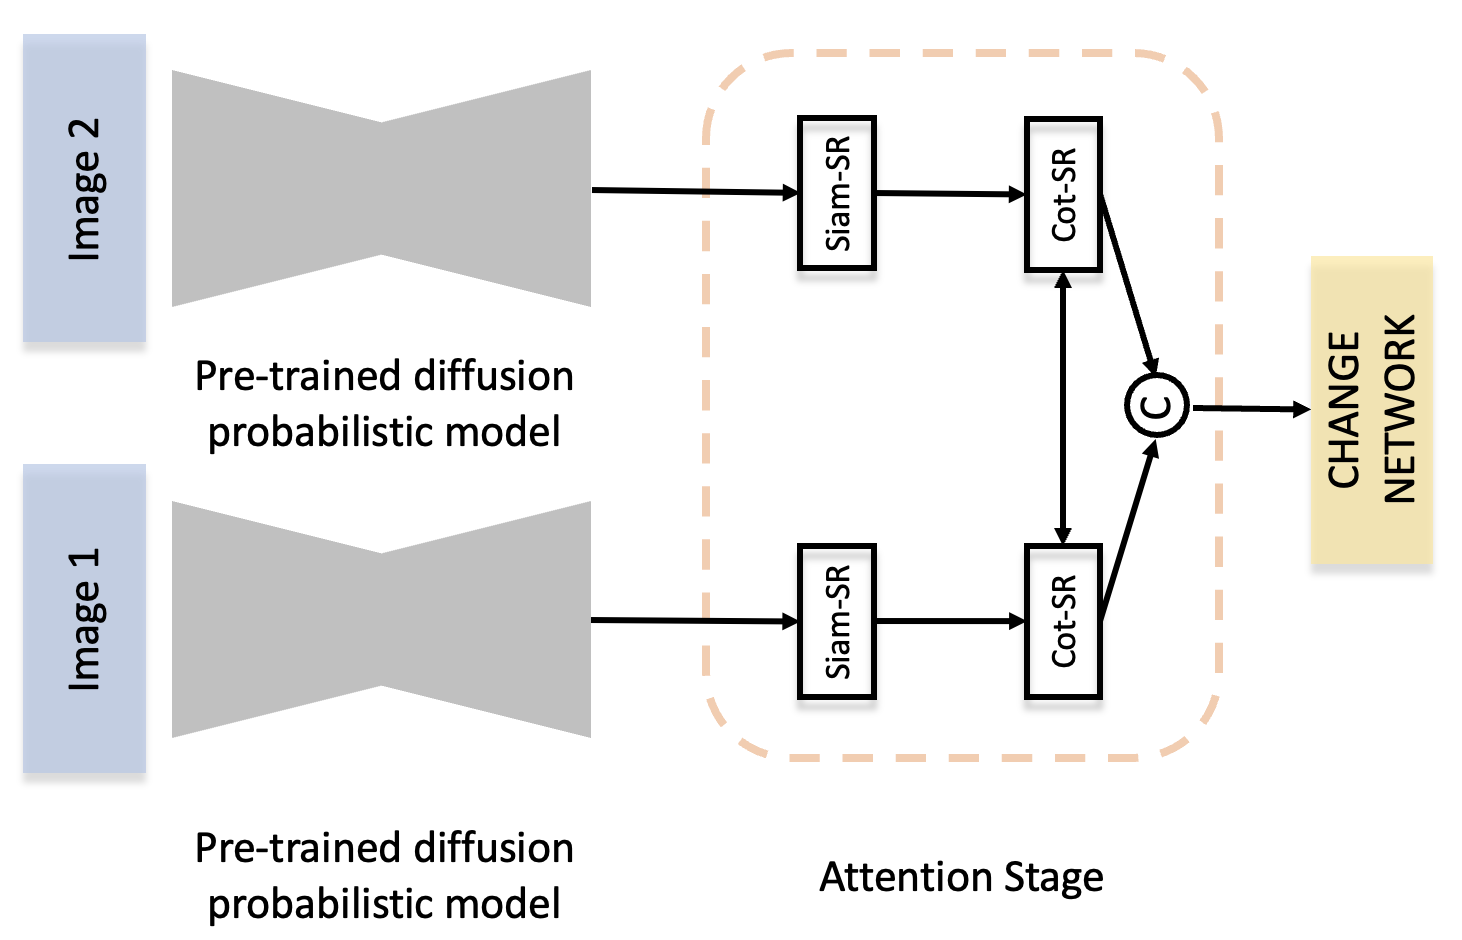
\includegraphics[width=\linewidth]{baseline_with_attention.png}
      \caption{Attention based model}
      \label{fig:baseline_with_attention}
  \end{subfigure}
  \hspace{0.1\textwidth}
  \begin{subfigure}[b]{0.4\linewidth}
      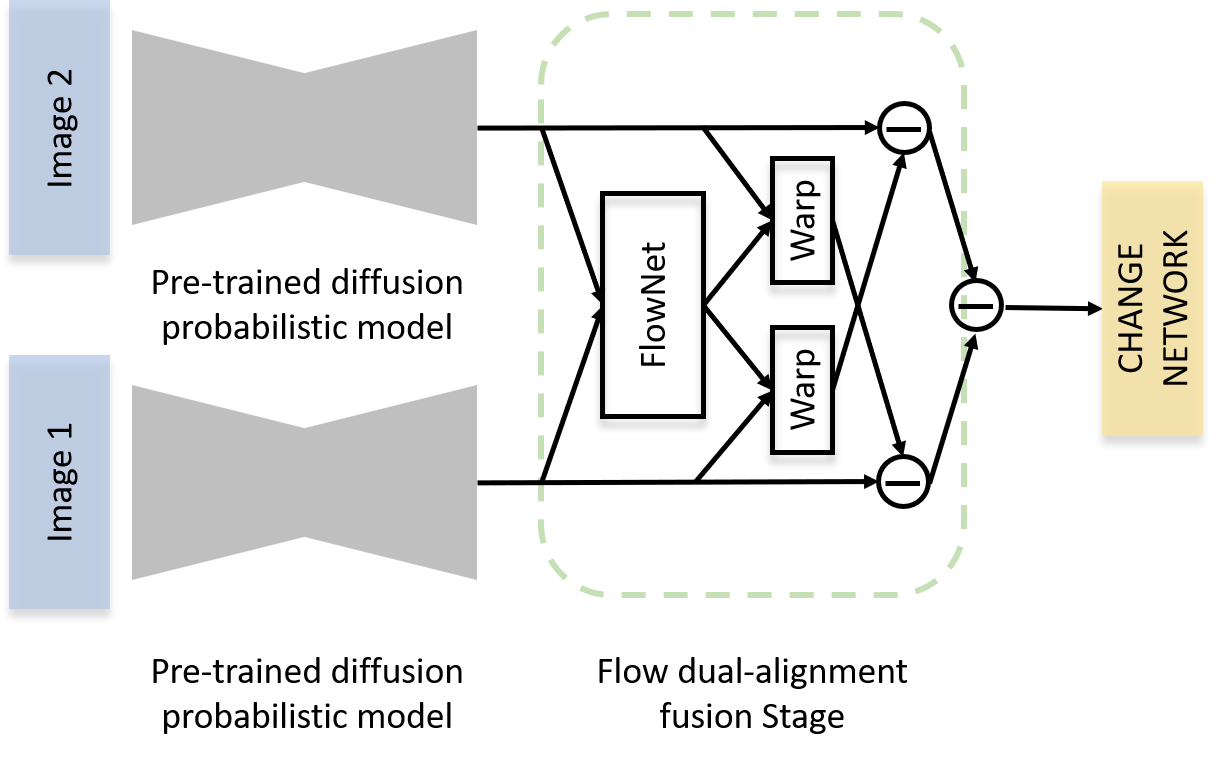
\includegraphics[width=\linewidth]{baseline_with_fdaf.png}
      \caption{FDAF based model}
      \label{fig:baseline_with_fdaf}
  \end{subfigure}
  \caption{Structure of the baseline model with attention and FDAF}
  \label{fig:baseline_with_attention_and_fdaf}
\end{figure}

\subsection{Feature Attention}

\subfile{subfiles/method_attention.tex}

\subsection{FDAF}

\subfile{subfiles/method_fdaf.tex}


\section{Experiment}

\subfile{subfiles/experiment.tex}


\section{Conclusion}

\subfile{subfiles/conclusion.tex}


\section{General formatting instructions}
\label{gen_inst}


The text must be confined within a rectangle 5.5~inches (33~picas) wide and
9~inches (54~picas) long. The left margin is 1.5~inch (9~picas).  Use 10~point
type with a vertical spacing (leading) of 11~points.  Times New Roman is the
preferred typeface throughout, and will be selected for you by default.
Paragraphs are separated by \nicefrac{1}{2}~line space (5.5 points), with no
indentation.


The paper title should be 17~point, initial caps/lower case, bold, centered
between two horizontal rules. The top rule should be 4~points thick and the
bottom rule should be 1~point thick. Allow \nicefrac{1}{4}~inch space above and
below the title to rules. All pages should start at 1~inch (6~picas) from the
top of the page.


For the final version, authors' names are set in boldface, and each name is
centered above the corresponding address. The lead author's name is to be listed
first (left-most), and the co-authors' names (if different address) are set to
follow. If there is only one co-author, list both author and co-author side by
side.


Please pay special attention to the instructions in Section \ref{others}
regarding figures, tables, acknowledgments, and references.


\section{Headings: first level}
\label{headings}


All headings should be lower case (except for first word and proper nouns),
flush left, and bold.


First-level headings should be in 12-point type.


\subsection{Headings: second level}


Second-level headings should be in 10-point type.


\subsubsection{Headings: third level}


Third-level headings should be in 10-point type.


\paragraph{Paragraphs}


There is also a \verb+\paragraph+ command available, which sets the heading in
bold, flush left, and inline with the text, with the heading followed by 1\,em
of space.


\section{Figures, tables, references}
\label{others}


These instructions apply to everyone.


\subsection{Footnotes}


Footnotes should be used sparingly.  If you do require a footnote, indicate
footnotes with a number\footnote{Sample of the first footnote.} in the
text. Place the footnotes at the bottom of the page on which they appear.
Precede the footnote with a horizontal rule of 2~inches (12~picas).


Note that footnotes are properly typeset \emph{after} punctuation
marks.\footnote{As in this example.}


\subsection{Figures}


\begin{figure}
  \centering
  \fbox{\rule[-.5cm]{0cm}{4cm} \rule[-.5cm]{4cm}{0cm}}
  \caption{Sample figure caption.}
\end{figure}


All artwork must be neat, clean, and legible. Lines should be dark enough for
purposes of reproduction. The figure number and caption always appear after the
figure. Place one line space before the figure caption and one line space after
the figure. The figure caption should be lower case (except for first word and
proper nouns); figures are numbered consecutively.


You may use color figures.  However, it is best for the figure captions and the
paper body to be legible if the paper is printed in either black/white or in
color.


\subsection{Tables}


All tables must be centered, neat, clean and legible.  The table number and
title always appear before the table.  See Table~\ref{sample-table}.


Place one line space before the table title, one line space after the
table title, and one line space after the table. The table title must
be lower case (except for first word and proper nouns); tables are
numbered consecutively.


Note that publication-quality tables \emph{do not contain vertical rules.} We
strongly suggest the use of the \verb+booktabs+ package, which allows for
typesetting high-quality, professional tables:
\begin{center}
  \url{https://www.ctan.org/pkg/booktabs}
\end{center}
This package was used to typeset Table~\ref{sample-table}.


\begin{table}
  \caption{Sample table title}
  \label{sample-table}
  \centering
  \begin{tabular}{lll}
    \toprule
    \multicolumn{2}{c}{Part}                   \\
    \cmidrule(r){1-2}
    Name     & Description     & Size ($\mu$m) \\
    \midrule
    Dendrite & Input terminal  & $\sim$100     \\
    Axon     & Output terminal & $\sim$10      \\
    Soma     & Cell body       & up to $10^6$  \\
    \bottomrule
  \end{tabular}
\end{table}

\subsection{Math}
Note that display math in bare TeX commands will not create correct line numbers for submission. Please use LaTeX (or AMSTeX) commands for unnumbered display math. (You really shouldn't be using \$\$ anyway; see \url{https://tex.stackexchange.com/questions/503/why-is-preferable-to} and \url{https://tex.stackexchange.com/questions/40492/what-are-the-differences-between-align-equation-and-displaymath} for more information.)

\subsection{Final instructions}

Do not change any aspects of the formatting parameters in the style files.  In
particular, do not modify the width or length of the rectangle the text should
fit into, and do not change font sizes (except perhaps in the
\textbf{References} section; see below). Please note that pages should be
numbered.

Of note is the command \verb+\cite+, which produces citations appropriate for
use in inline text.  For example,
\begin{verbatim}
   Graphaf~\cite{shi2020graphaf}
\end{verbatim}
produces
\begin{quote}
  Graphaf~\cite{shi2020graphaf}.
\end{quote}

\newpage


\bibliographystyle{splncs04}
\bibliography{reference}

\end{document}